\documentclass{beamer}
\usepackage{pgfpages}
\usepackage[backend=bibtex]{biblatex}
\usepackage{multicol}
\usepackage{multimedia}
\usepackage[absolute,overlay]{textpos}
\usepackage{parskip}
\usepackage{hyperref}
\usepackage{lmodern}
\hypersetup{colorlinks=true, urlcolor=blue}
\setlength{\parskip}{\smallskipamount} 
%\usepackage[texcoord,grid,gridunit=mm,gridcolor=red!10,subgridcolor=green!10]{eso-pic} %DELETE when done with grid
\setbeameroption{hide notes} % Only slides
%\setbeameroption{show only notes} % Only notes
%\setbeameroption{show notes on second screen=right} % Both
%\bibliography{../../papers/references.bib}
\setbeamerfont{footnote}{size=\tiny}
%\AtEveryCitekey{\clearfield{title}}

%
% Choose how your presentation looks.
%
% For more themes, color themes and font themes, see:
% http://deic.uab.es/~iblanes/beamer_gallery/index_by_theme.html
%
\mode<presentation>
{
  \usetheme{Warsaw}      % or try Darmstadt, Madrid, Warsaw, ...
  \usecolortheme{default} % or try albatross, beaver, crane, ...
  \usefonttheme{default}  % or try serif, structurebold, ...
  \setbeamertemplate{navigation symbols}{}
  \setbeamertemplate{caption}[numbered]
} 

\usepackage[english]{babel}
%\usepackage[utf8x]{inputenc} %Doesn't play well with biblatex
\usepackage{amssymb}
\usepackage{bm}
\usepackage{color}
\usepackage{graphicx}

\newcommand{\red}[1]{{\color{red}{#1}}}

\title[{\color{white}{Intro}}]{{\Huge Introduction} \\ {\normalsize Clubes de Ciencia - Ensenada 2017 \\ Frank Wilzcek Course}}
\author{Cody Petrie \& David Rojas}
\institute{Universidad Aut\'onoma de Baja California}
\date{}
\titlegraphic{\includegraphics[width=2cm]{../../logos/CdeC_logo.png}~%\hspace*{0.75cm}~
   \includegraphics[width=1.5cm]{../../logos/UABC_logo.png}
}

\begin{document}

%\setbeamertemplate{frametitle}[default][center]
\begin{frame}
   \titlepage
\end{frame}

% Uncomment these lines for an automatically generated outline.
%\begin{frame}{Outline}
%  \tableofcontents
%\end{frame}

% Commands to include a figure:
%\begin{figure}
%\includegraphics[width=\textwidth]{your-figure's-file-name}
%\caption{\label{fig:your-figure}Caption goes here.}
%\end{figure}

\begin{frame}{Clubes de Ciencia}
   \begin{itemize}
      \item In this class we're going to learn how to use technology to augment our understanding of the world around us.
      \item We are going to learn about \ldots
      \begin{itemize}
         \item Computer programming with Python
         \item Circuit building and Arduino
         \item Methods for learning about the world around us
      \end{itemize}
      \item We want to make sure that you get what you want out of this class \ldots what do you guys want out of this course?
   \end{itemize}
\end{frame}

\begin{frame}{Clubes de Ciencia}
   \begin{itemize}
      \item To get your Diploma you need to \ldots
      \begin{itemize}
         \item ``Full attendance" which means you participate everyday (if you have to miss a day that's okay, just let us know).
         \item Complete intro survey on your CdeC profile (We'll do this in a minute)
         \item Complete exit survey on your CdeC profile which becomes available on Saturday.
      \end{itemize}
   \end{itemize}
\end{frame}

\begin{frame}{Clubes de Ciencia}
   \begin{center}
      \Huge \textcolor{blue}{Complete Survey}
   \end{center}
\end{frame}

\begin{frame}{Cody}
   \begin{center}
      \Huge \textcolor{blue}{Introducing Cody}
   \end{center}
\end{frame}

\begin{frame}{Cody - Family}
   \begin{itemize}
      \item Undergraduate degree from BYU in Physics with a minor in Astronomy. Now I'm in physics PhD program at ASU.
      \item There I met my beautiful wife and we got married. I got her to fall in love with my by putting spanish love notes on her car while she was working or at school :)
      \item We have three kids, Ammon (4.9), Cooper (3) and Olivia (0.5)
   \end{itemize}
   \begin{center}
      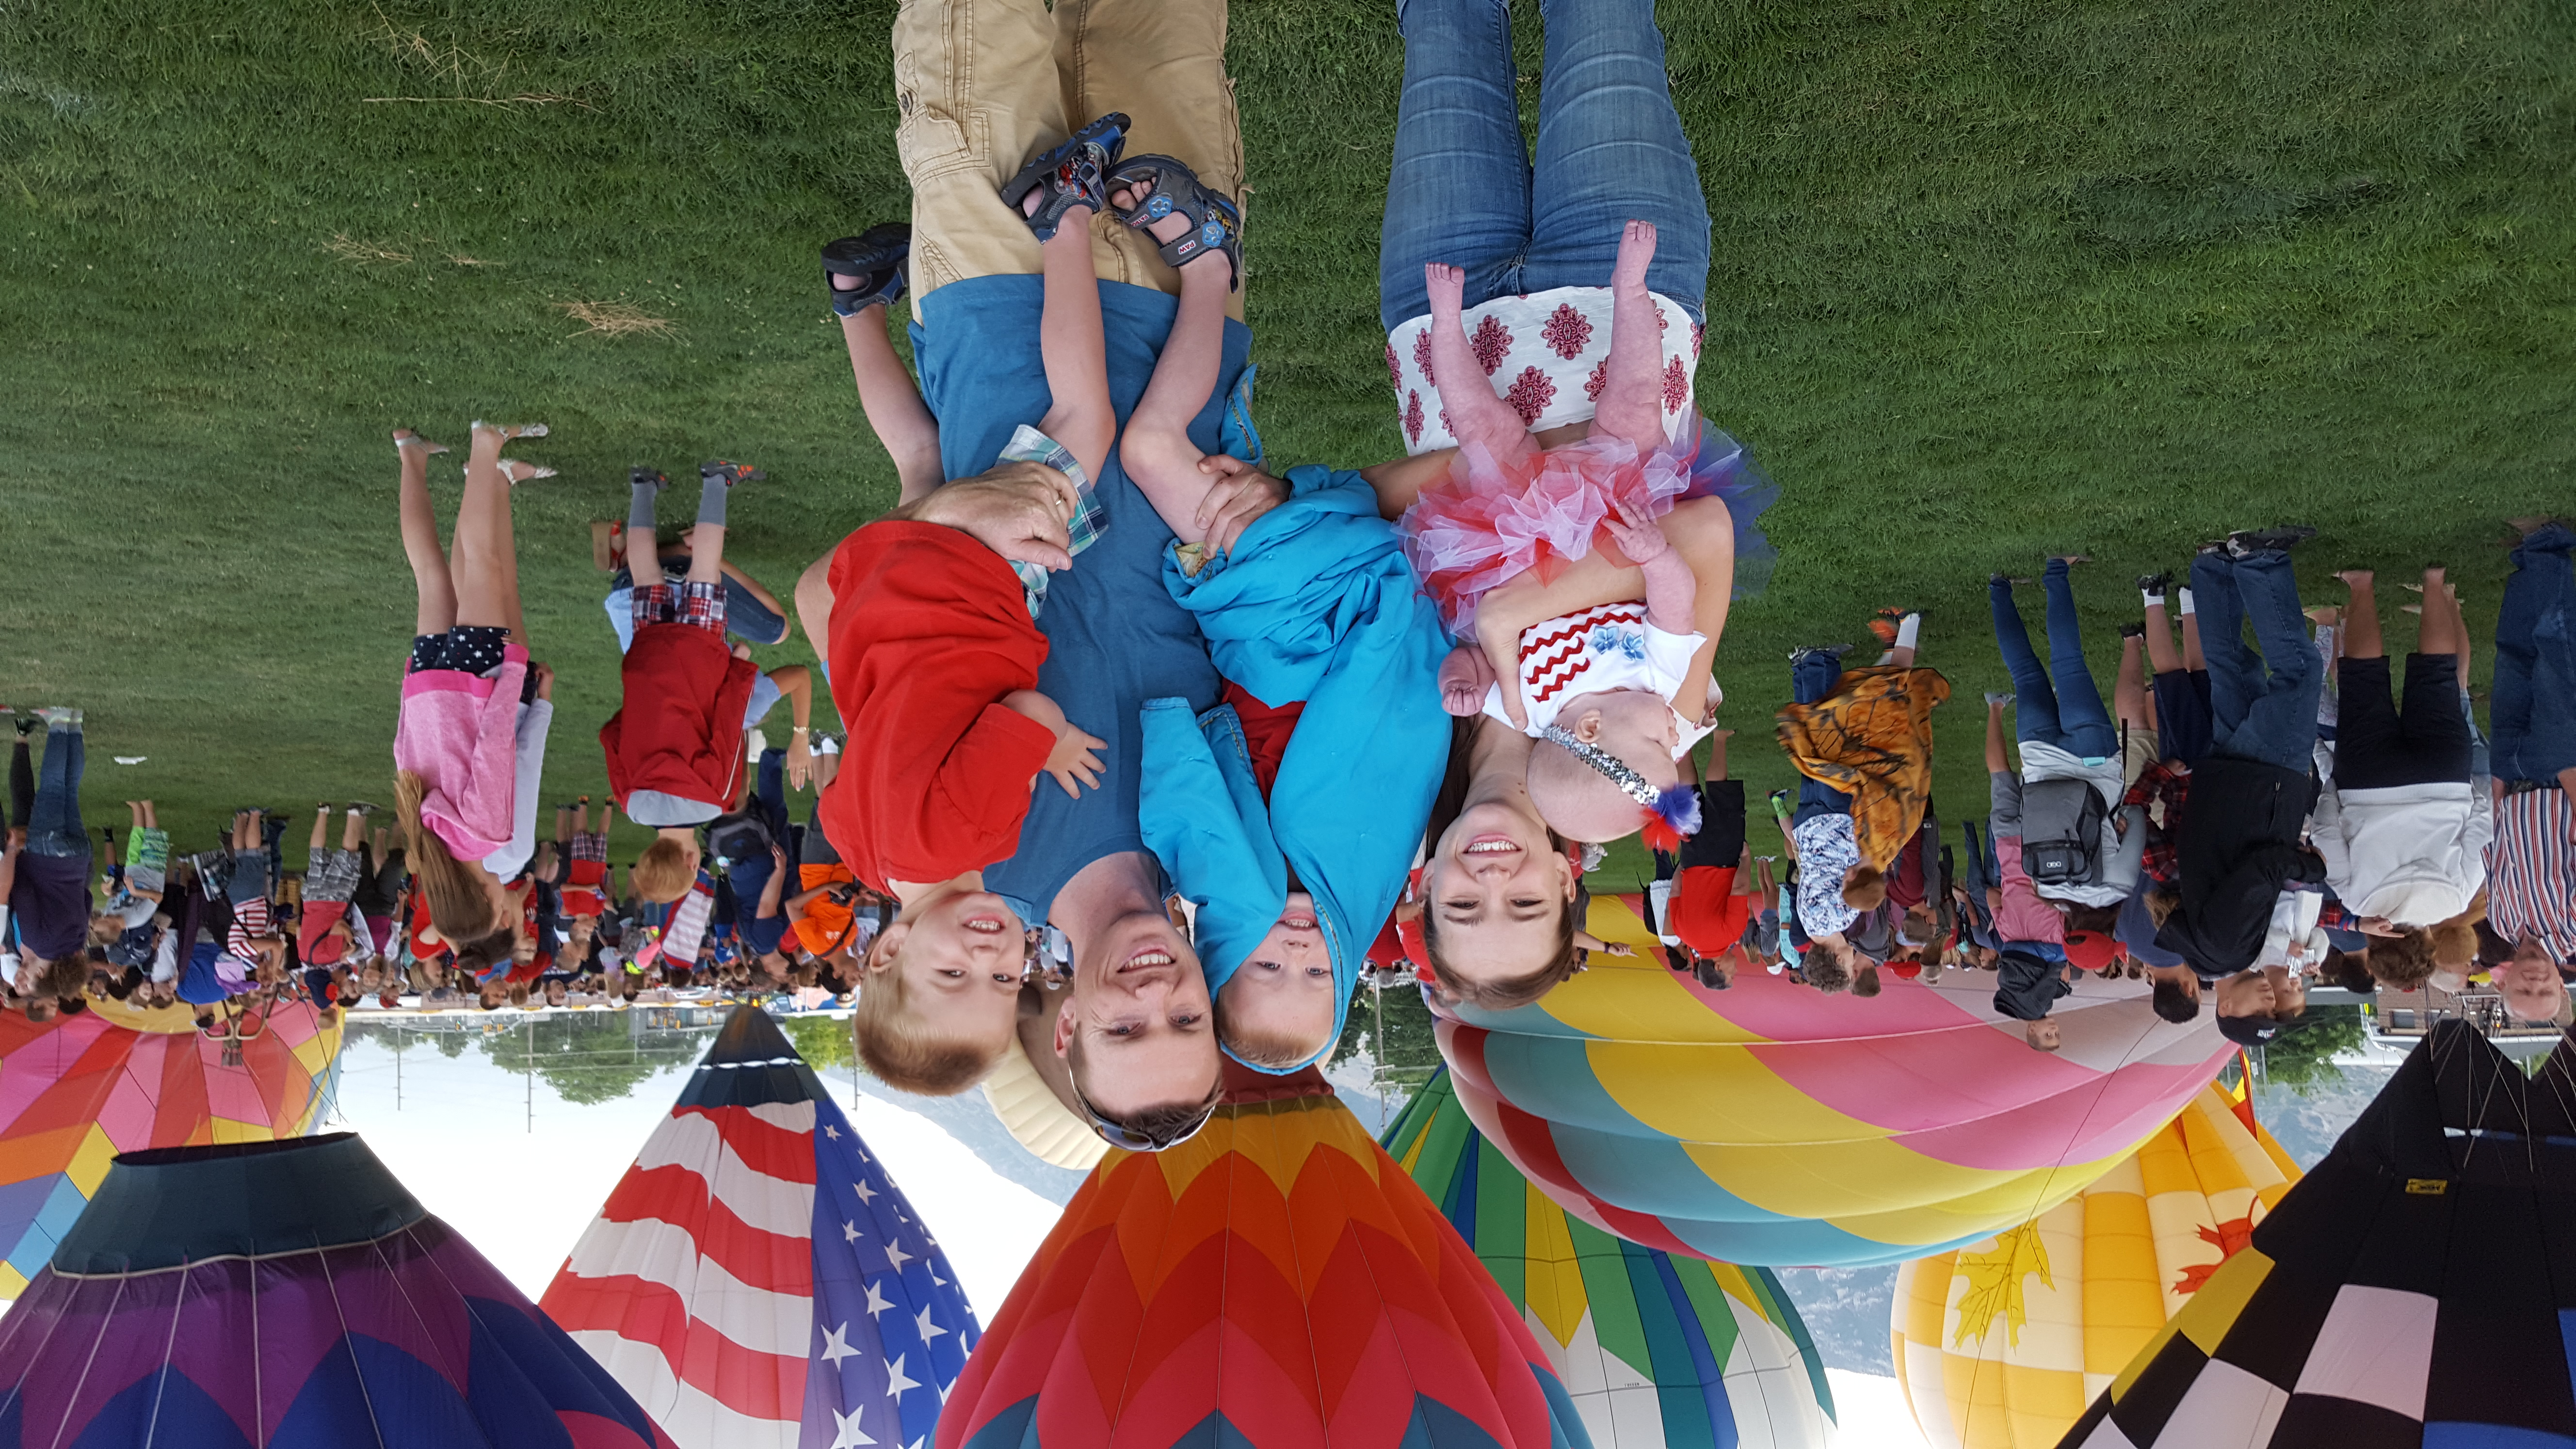
\includegraphics[width=0.5\textwidth, angle=180, origin=c]{figures/family1.jpg}
      ~ ~
      \includegraphics[width=0.5\textwidth]{figures/family2.jpg}
   \end{center}
\end{frame}

\begin{frame}{Cody - Hobbies}
   \begin{textblock*}{\textwidth}(0.3cm,0.8cm) % {block width} (coords)
      \includegraphics[width=4.0cm]{figures/radio.jpg}
   \end{textblock*}
   \begin{textblock*}{\textwidth}(4.5cm,0.8cm) % {block width} (coords)
      \includegraphics[width=3.5cm]{figures/camping.jpg}
   \end{textblock*}
   \begin{textblock*}{\textwidth}(0.3cm,3.3cm) % {block width} (coords)
      \includegraphics[width=3.5cm]{figures/fishing.jpg}
   \end{textblock*}
   \begin{textblock*}{\textwidth}(8.5cm,0.8cm) % {block width} (coords)
      \includegraphics[width=3.5cm]{figures/hiking.jpg}
   \end{textblock*}
   \begin{textblock*}{\textwidth}(0.3cm,6.3cm) % {block width} (coords)
      \includegraphics[width=3.5cm]{figures/rafting.jpg}
   \end{textblock*}
   \begin{textblock*}{\textwidth}(8.5cm,6.3cm) % {block width} (coords)
      \includegraphics[width=3.5cm]{figures/skiing.jpg}
   \end{textblock*}
   \begin{textblock*}{\textwidth}(4.4cm,6.1cm) % {block width} (coords)
      \includegraphics[width=3.8cm]{figures/ziggy.jpg}
   \end{textblock*}
\end{frame}

\begin{frame}{Cody - Research}
   \begin{itemize}
      \item Computational Nuclear Physics.
      \begin{itemize}
         \item Quantum Monte Carlo methods to solve for energies of nuclear systems like $^4$He, $^{16}$O, $^{40}$Ca and symmetric nuclear matter.
         \begin{equation}
            E = \int dx_1 \int dy_1 \ldots \int dz_N \Psi^*(R,t) H \Psi(R,t)
         \end{equation}
         \item This is a lot of integrals over complicated things... $\Psi$ is complicated and $H$ is complicated.
         \item So we ``cheat" and use Monte Carlo methods!
      \end{itemize}
      \begin{center}
         \includegraphics[width=0.5\textwidth]{figures/dice.jpg}
      \end{center}
   \end{itemize}
\end{frame}

\begin{frame}{Cody - Monte Carlo Integration}
   \begin{itemize}
      \item If you wanted to know the area of a circle you would integrate
      \begin{equation}
         A = \int \int_{x^2+y^2\le r} dx dy = \int_0^{2\pi} \int_0^r r' dr' d\theta
      \end{equation}
      \item Or you could use Monte Carlo integration where $A=\frac{N_{circle}}{N_{total}}A_{square}$.
      \begin{center}
         \includegraphics[width=0.5\textwidth]{figures/circle.png}
      \end{center}
   \end{itemize}
\end{frame}

\begin{frame}{David}
   \begin{center}
      \Huge \textcolor{blue}{Introducing David}
   \end{center}
\end{frame}

\begin{frame}{David}
   \begin{itemize}
      \item Ingeniero en Nanotecnolog\'ia, por parte de la Universidad Aut\'onoma de Baja California. Este Septiembre ingresar\'e a la Maestr\'ia en \'Optica del CICESE.
      \item Soy originario de Durango, M\'exico.
      \item En la Preparatoria la escuela me parec\'ia aburrida y al salir de \'esta ingres\'e al Ej\'ercito Mexicano por un a\~no.
   \end{itemize}
   ~\\~\\~\\~\\~\\~\\~\\~\\~\\~\\~\\~\\
   \begin{textblock*}{\textwidth}(0.3cm,4.5cm) % {block width} (coords)
      \includegraphics[width=3.0cm]{figures/UABC_logo.jpg}
   \end{textblock*}
   \begin{textblock*}{\textwidth}(3.5cm,4.7cm) % {block width} (coords)
      \includegraphics[width=3.7cm]{figures/nach.png}
   \end{textblock*}
   \begin{textblock*}{\textwidth}(6.35cm,7.1cm) % {block width} (coords)
      \includegraphics[width=3.0cm]{figures/cicese_logo.png}
   \end{textblock*}
   \begin{textblock*}{\textwidth}(7.4cm,5.6cm) % {block width} (coords)
      \includegraphics[width=1.0cm]{figures/optica.jpg}
   \end{textblock*}
   \begin{textblock*}{\textwidth}(9.4cm,4.3cm) % {block width} (coords)
      \includegraphics[width=3.0cm]{figures/military.png}
   \end{textblock*}
\end{frame}

\begin{frame}{David - Hobbies}
   \begin{textblock*}{\textwidth}(0.3cm,1.5cm) % {block width} (coords)
      \includegraphics[width=3.0cm]{figures/sae_david.png}
   \end{textblock*}
   \begin{textblock*}{\textwidth}(3.6cm,1.0cm) % {block width} (coords)
      \includegraphics[width=4.0cm]{figures/galaxy.png}
   \end{textblock*}
   \begin{textblock*}{\textwidth}(7.9cm,2.0cm) % {block width} (coords)
      \includegraphics[width=1.5cm]{figures/sae_logo.png}
   \end{textblock*}
   \begin{textblock*}{\textwidth}(9.7cm,1.0cm) % {block width} (coords)
      \includegraphics[width=3.0cm]{figures/gatos.jpg}
   \end{textblock*}
   \begin{textblock*}{\textwidth}(0.3cm,5.5cm) % {block width} (coords)
      \includegraphics[width=4.3cm]{figures/sae_group.png}
   \end{textblock*}
   \begin{textblock*}{\textwidth}(4.9cm,6.2cm) % {block width} (coords)
      \includegraphics[width=3.3cm]{figures/fibopt.png}
   \end{textblock*}
   \begin{textblock*}{\textwidth}(8.5cm,6.0cm) % {block width} (coords)
      \includegraphics[width=4.0cm]{figures/camping_david.png}
   \end{textblock*}
\end{frame}

\begin{frame}{David - Research}
   \begin{textblock*}{\textwidth}(0.3cm,1.0cm) % {block width} (coords)
      \includegraphics[width=6.0cm]{figures/intref.png}
   \end{textblock*}
   \begin{textblock*}{\textwidth}(3.3cm,4.2cm) % {block width} (coords)
      \includegraphics[width=7.0cm]{figures/mixing.png}
   \end{textblock*}
   \begin{textblock*}{\textwidth}(6.8cm,1.0cm) % {block width} (coords)
      \includegraphics[width=5.0cm]{figures/laser.jpg}
   \end{textblock*}
\end{frame}

\begin{frame}{David - Future research in Master and PhD}
   \begin{center}
      \includegraphics[width=\textwidth]{figures/quantum.png}
   \end{center}
\end{frame}

\begin{frame}{Rompahielos}
   \begin{itemize}
      \item Two-truths and one lie?
   \end{itemize}
\end{frame}

\begin{frame}{Picture Citations}
\fontsize{5}{4}\selectfont 
CdeC logo (accessed 13 July 2017): \href{https://www.clubesdeciencia.mx}{https://www.clubesdeciencia.mx}\\
UABC logo (accessed 13 July 2017): \href{http://www.uabc.mx/}{http://www.uabc.mx/}\\
Dice (accessed 24 July 2017): \href{http://www.thelegalintelligencer.com/image/EM/PA/rolling\_dice-Article-201504021454.jpg}{http://www.thelegalintelligencer.com/image/EM/PA/rolling\_dice-Article-201504021454.jpg}\\
Monte Carlo Integration (accessed 24 July 2017): \href{https://en.wikipedia.org/wiki/Monte\_Carlo\_integration}{https://en.wikipedia.org/wiki/Monte\_Carlo\_integration}\\
CICESE logo (accessed 24 July 2017): \href{http://posgrados.cicese.mx/logos/logos}{http://posgrados.cicese.mx/logos/logos}\\
UABC logo (accessed 24 July 2017): \href{http://www.uabc.mx/logos}{http://www.uabc.mx/logos}\\
Spontaneus Four Wave Mixing (accessed 24 July 2017): \href{http://biomedicaloptics.spiedigitallibrary.org/data/journals/biomedo/934300/jbo\_20\_8\_086006\_f001.png}{http://biomedicaloptics.spiedigitallibrary.org/data/journals/biomedo/934300/jbo\_20\_8\_086006\_f001.png}\\
Pulsed Laser (accessed 24 July 2017): \href{http://img.directindustry.com/images\_di/photo-m2/27505-2826745.jpg}{http://img.directindustry.com/images\_di/photo-m2/27505-2826745.jpg}\\
Fiber Optics (accessed 24 July 2017): \href{http://cdn4.explainthatstuff.com/fiber-optics-total-internal-reflection.png}{http://cdn4.explainthatstuff.com/fiber-optics-total-internal-reflection.png}\\
Quantum computing (accessed 24 July 2017): \href{http://kubrickgroup.com/wp-content/uploads/2016/12/Quatum\_pic.png}{http://kubrickgroup.com/wp-content/uploads/2016/12/Quatum\_pic.png}\\
\end{frame}

\end{document}
